\begin{center}
\LARGE
Prøve
\end{center}
\stepcounter{section}

\begin{opgavetekst}{Opgave 1}
	\begin{center}
		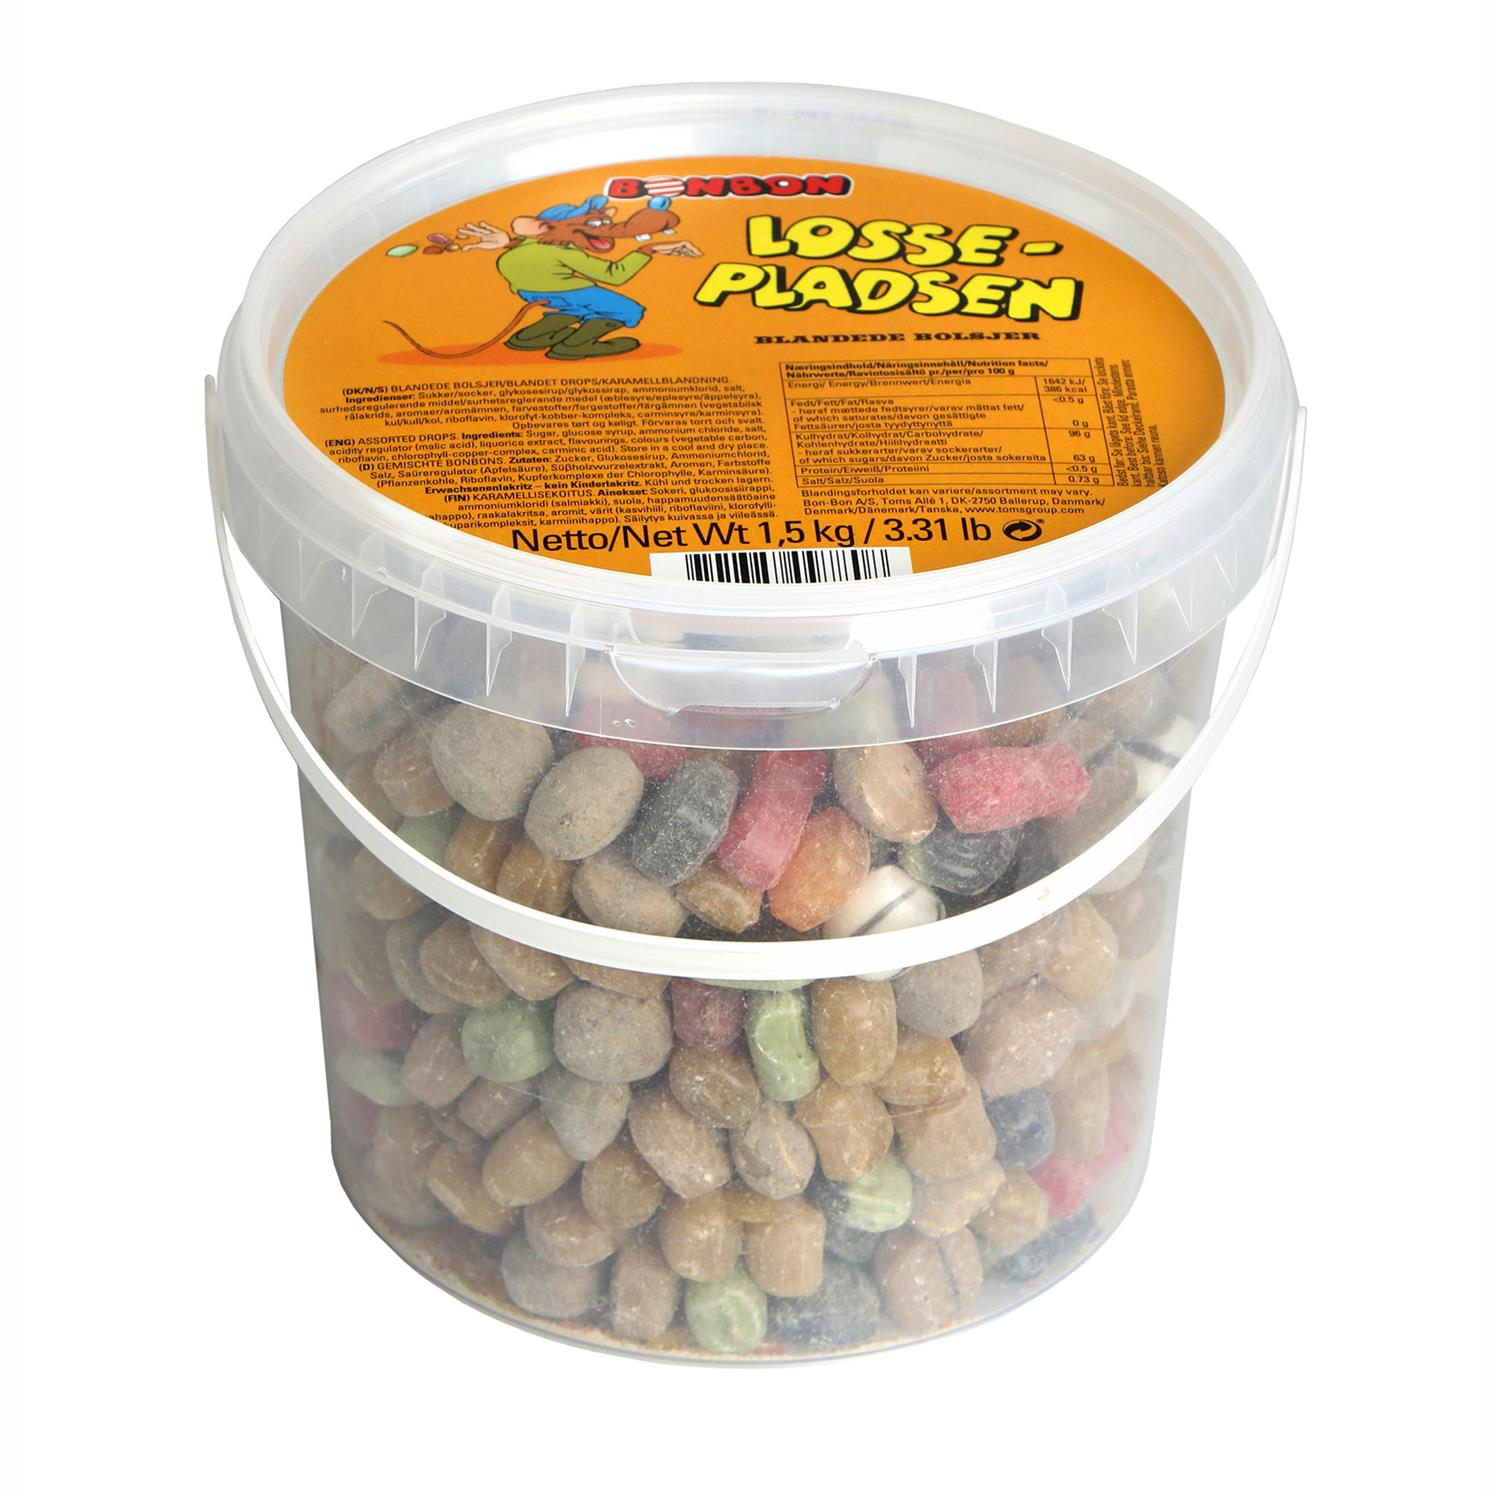
\includegraphics[width=0.4\textwidth]{Billeder/Losseplads.jpg}
	\end{center}
	Producenten af en bestemt type bolscher sælger beholdere á 1500g med bolscher. En grundig stikprøve har vist, at nettovægten af beholderne er normalfordelt med 
	en middelværdi på 1506g og en spredning på 11g. 
\end{opgavetekst}
\begin{delopgave}{(10 point)}{1}
	Afgør, om en beholder med en nettovægt på 1538g er et exceptionelt udfald. 
\end{delopgave}
\begin{meretekst}
	Lad $f$ være tæthedsfunktionen for den stokastiske variabel, der beskriver nettovægten af en beholder med bolscher.
\end{meretekst}
\begin{delopgave}{(10 point)}{2}
	Opskriv et integral, der beskriver sandsynligheden for at få en beholder med en nettovægt på mere end 1510g.
\end{delopgave}

%%%%%%%%%%%%%%%%%%%%%%%%%%%%%%%%%%%%%%%%%%%%%%%%%%%%%%%%%%%%%%%%%%%%%%%
%							Ny Opgave!!!!!							%
%%%%%%%%%%%%%%%%%%%%%%%%%%%%%%%%%%%%%%%%%%%%%%%%%%%%%%%%%%%%%%%%%%%%%%%

\begin{opgavetekst}{Opgave 2}
	En funktion $f:\mathbb{R}^2 \to \mathbb{R}$ er givet ved
	\begin{align*}
		f(x,y) = 2x^2-4x-2y^2+8y.
	\end{align*}
	Funktionen $f$ har netop ét stationært punkt.
\end{opgavetekst}
\begin{delopgave}{(10 point)}{1}
	Bestem det stationære punkt for $f$. 
\end{delopgave}

%%%%%%%%%%%%%%%%%%%%%%%%%%%%%%%%%%%%%%%%%%%%%%%%%%%%%%%%%%%%%%%%%%%%%%%
%							Ny Opgave!!!!!							%
%%%%%%%%%%%%%%%%%%%%%%%%%%%%%%%%%%%%%%%%%%%%%%%%%%%%%%%%%%%%%%%%%%%%%%%

\newpage

\begin{opgavetekst}{Opgave 3}
	En vektorfunktion $\vv{r}:\mathbb{R}\to \mathbb{R}^2$ er givet ved
	\begin{align*}
		\vv{r}(t) = 
		\begin{pmatrix}
			t^2-4 \\
			t^2-6t-3
		\end{pmatrix}.
	\end{align*}
\end{opgavetekst}
\begin{delopgave}{(10 point)}{1}
	Bestem de to skæringspunkter mellem parameterkurven for $\vv{r}$ og $y$-aksen.
\end{delopgave}
\begin{delopgave}{(10 point)}{2}
	Bestem det punkt, hvor parameterkurven for $\vv{r}$ har en vandret tangent. 
\end{delopgave}

%%%%%%%%%%%%%%%%%%%%%%%%%%%%%%%%%%%%%%%%%%%%%%%%%%%%%%%%%%%%%%%%%%%%%%%
%							Ny Opgave!!!!!							%
%%%%%%%%%%%%%%%%%%%%%%%%%%%%%%%%%%%%%%%%%%%%%%%%%%%%%%%%%%%%%%%%%%%%%%%

\begin{opgavetekst}{Opgave 4}
	En funktion $f:\mathbb{R} \to \mathbb{R}$ er givet ved
	\begin{align*}
		f(x) = -\cos(4x^3+13)12x^2.
	\end{align*}
\end{opgavetekst}
\begin{delopgave}{(10 point)}{1}
	Udregn det ubestemte integral $I$ givet ved
	\begin{align*}
		I = \int f(x) dx.
	\end{align*}
\end{delopgave}

%%%%%%%%%%%%%%%%%%%%%%%%%%%%%%%%%%%%%%%%%%%%%%%%%%%%%%%%%%%%%%%%%%%%%%%
%							Ny Opgave!!!!!							%
%%%%%%%%%%%%%%%%%%%%%%%%%%%%%%%%%%%%%%%%%%%%%%%%%%%%%%%%%%%%%%%%%%%%%%%


\begin{opgavetekst}{Opgave 5}
	En funktion $f$ er løsning til differentialligningen
	\begin{align*}
		y' = 30 + 6y
	\end{align*}
\end{opgavetekst}
\begin{delopgave}{(10 point)}{1}
	Bestem en ligning for tangenten til grafen for $f$ gennem punktet $P(1,-4)$.
\end{delopgave}
\begin{delopgave}{(10 point)}{2}
	Bestem den partikulære løsning til differentialligningen, hvis graf skærer gennem punktet $Q(0,-2)$.
\end{delopgave}

%%%%%%%%%%%%%%%%%%%%%%%%%%%%%%%%%%%%%%%%%%%%%%%%%%%%%%%%%%%%%%%%%%%%%%%
%							Ny Opgave!!!!!							%
%%%%%%%%%%%%%%%%%%%%%%%%%%%%%%%%%%%%%%%%%%%%%%%%%%%%%%%%%%%%%%%%%%%%%%%
